\chapter{Implementation}\label{ch:impl}

\section{The Dataflow Model extended}\label{sec:impl:dataflow}

While the Dataflow paper \cite{Akidau:2015} summarised in \cref{sec:prep:dataflow} gives an overview of the Dataflow Model, it does not provide sufficient detail for its full implementation.
This section draws on many sources, including the Apache Beam codebase, the Apache JIRA issue tracker, and the Apache Beam mailing list in order to compile the extensions to the model necessary for a full, working implementation.

It is important to note that many concepts in the Beam codebase are specific to the Java implementation.
Where the author felt this was the case, a more general concept was defined.
The need to implement these concepts in the very different Elixir language served as a good benchmark of which concepts were implementation details rather than necessary model changes.
The implementation details of the Elixir implementation are described later in this chapter.

Keeping the previous paragraph in mind, as well as the fact that the Beam project is an active project which is constantly evolving, it is important to note that this chapter does not aim to provide a full description of the Beam Model as it stands today.
Rather, it takes direction and inspiration therefrom to produce a self-consistent extension to the Dataflow Model which enables implementations of it to be built taking a similar approach to Apache Beam.

Finally, the project tackles only the data processing model itself.
Further extensions to the model are necessary, and present in the Beam codebase, in order to enable easy, automated and efficient distribution of execution across a compute cluster.
These include checkpointing, serialisation and partitioning of data, but in themselves form a complex topic worthy of separate discussion.
Nevertheless, these concerns are outside the scope of this project and will only be mentioned tangentially where relevant.

\subsection{Pipelines, Transforms and Collections}\label{sec:impl:dataflow:pipelines-transforms-collections}

Pipelines are independent ``namespaces'' of computation.
They are essentially DAGs representing the flow of data through the system as it is transformed.

\begin{figure}[t]
	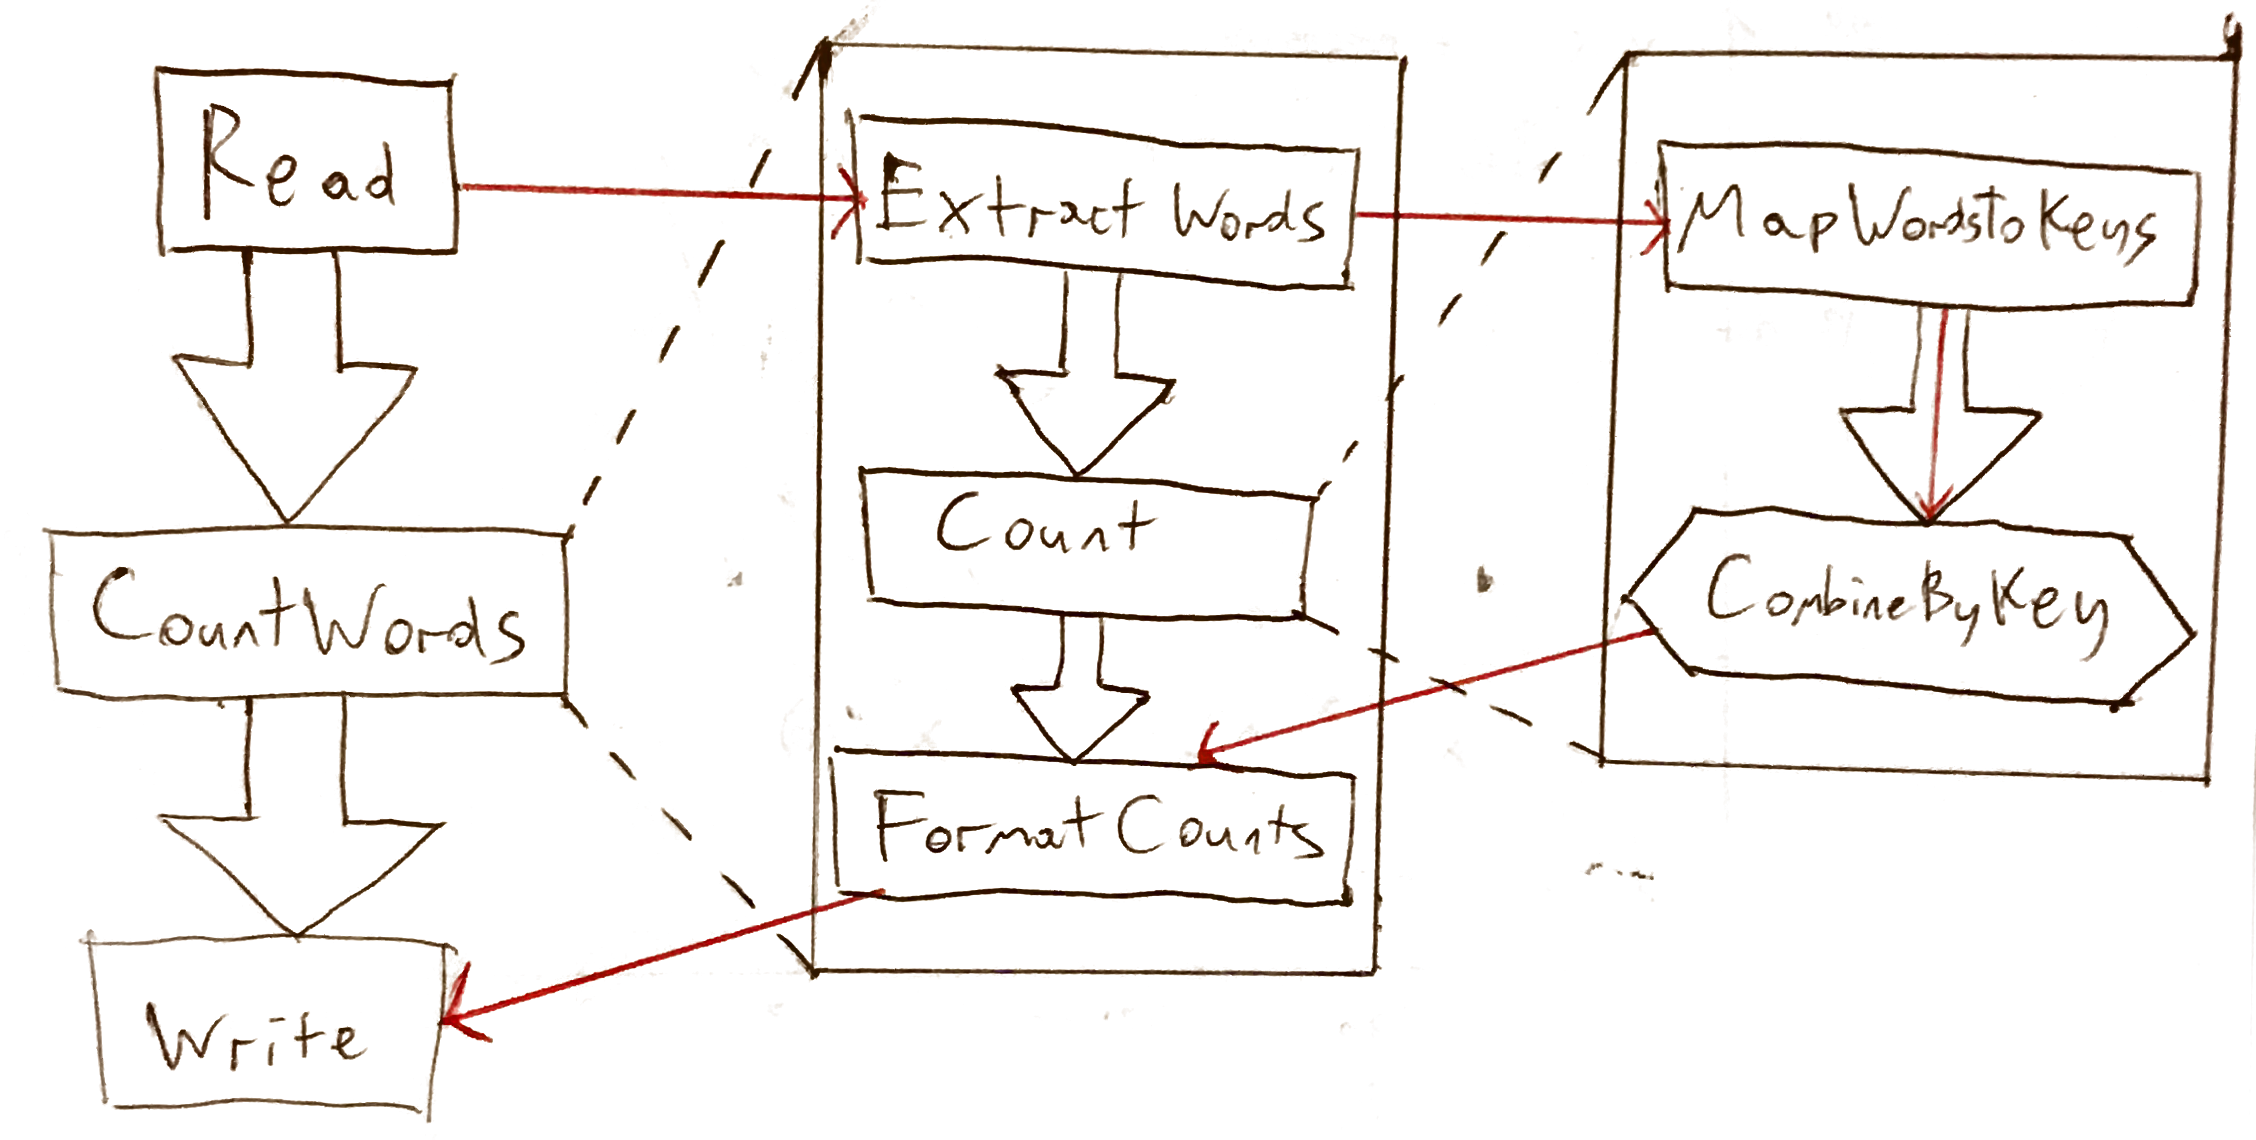
\includegraphics[width=\textwidth]{images/temp/composite-example}
	\caption{An example of a Pipeline utilising composite Transforms. The large arrows indicate the conceptual data flow path. The user expects to see visualisations or statistics using this abstraction. The red edges indicate the actual execution-time data flow---only leaf Transforms are actually instantiated and exchange data.}
	\label{fig:impl:composite-transforms}
\end{figure}

Each node in this graph is a Transform.\footnote
{
In the Beam documentation and various other literature, these objects are called PTransforms and PCollections (with ``P'' standing for ``parallel'').
In this document, they are simply referred to as Transforms and Collections, always capitalised.
}
Transforms can have multiple inputs or outputs.

Each edge in the graph represents a Collection.
This is a notion of the data flowing between Transforms.
Collections can be thought of as the description of all the data that will ever flow out of a particular transform.
The way we construct a Pipeline is by applying Transforms to Collections, the result being another, new Collection (or a structure grouping multiple new Collections).
This Collection encodes various information about the data, depending on the implementation, but among the more important data are the windowing strategy that the collection will follow, used by windowing transforms, which Transform produces the Collection, and the type of the data which will be produced.

Transforms may be primitive or composite---a primitive Transform is directly executed by the pipeline runner, while a composite Transform ``expands'' into multiple sub-Transforms at execution.
This is illustrated in \cref{fig:impl:composite-transforms}.
Different runners may choose to implement different Transforms as primitives and provide composite implementations for the rest.
They do this in a process called \emph{graph surgery}, performed before they start executing the Pipeline.

Composite Transforms are tracked for informational purposes (statistics, logging or visualisation), but don't actually get instantiated at execution time.
The existence of composite Transforms is one of the reasons it is important to track the producer of each Collection---the true producer may be within a nested tree of Transforms rather than being the Transforms we applied directly to the input Collection.


\todo{fix terminology about the below and refactor this section to keep it consistently---easy to get the concepts confused.}

There are three distinct types of entities which could reasonably be called Transforms.
The first is the class instance or structure which holds the parameters for the representation of the Transform and references its code at build-time.
This is what we actually \emph{apply} to a Collection.

The result of such an application is a new Collection.
However, as a side effect, a node representing a particular instance of the Transform in a tree, with particular inputs and outputs, is added to the DAG.
We call such a node an \emph{Applied Transform}.
As well as the parameters of the Transform that was applied, it holds extra information which will be used at execute-time.

Finally, at execute-time, this Applied Transform will be instantiated into some runtime structure which is responsible for actually performing computation.
This may be an object in the case of Java or an actor process in the case of Elixir.
In any case we will call such an instance a \emph{Transform Executor}.

\subsubsection{Collections and streams}

We say that data is \emph{added} to a Collection whenever its producing Transform Executor outputs data.
The Beam implementation explicitly tracks Collections, with Transform Executors really adding data to an in-memory object before it is dispatched as input to other Transform Executors.
The data is groped in \emph{bundles}, which also provide a convenient primitive for serialisation and checkpointing.

The Elixir implementation takes a different approach, with data flowing directly between Transform Executors using message passing.
Collections are used only to set up these links and do not exist at execution time.
The messages sent still contain lists of elements and not individual elements for efficiency.
This is explored further in \cref{todo}.

This illustrates the fact that although we conceptually think of streams of data flowing between Transform Executors, in practice the data is sent and processed in chunks.
The size of these chunks, amongst other factors, can determine where on the spectrum between batch, micro-batch and stream processing a particular runner lies.

\todo{discuss runners somewhere!!}

\subsubsection{Side inputs}

\todo{verify this definition is precise (or don't mention it)}

The Beam implementation has a concept of \emph{side inputs}, which are essentially views of Collections accessible to Transforms to aid in their processing.
For example, a branch of our pipeline processing game messages could identify abusive users and pass the current list as a side input to another Transform which uses this list to remove certain messages from the feed.
This means that the side input is not necessarily a stream of concurrent data as another input would be, but merely a convenient materialisation of data calculated elsewhere.
While being a useful concept, it was not implemented in this project and is not considered further in this document, mostly because of space and time concerns.


\subsection{Windows and panes}\label{sec:impl:dataflow:windows-panes}

As described in \cref{sec:prep:dataflow:where}, \emph{windows} are a concept used to group elements in event time (i.e.\ with regards to their intrinsic timestamps).
In practice, a window is merely a meta-value acting as a second key by which elements are grouped.
In the Beam and Elixir implementations, only two types of windows are present: the global window, encompassing all time and all elements, and the interval window, encompassing a specific period of time.
The only further requirement we make of a window value is that we be able to obtain the maximal time of an element which is still within that window (the maximal timestamp for the global window, and the inclusive upper bound for an interval window).

\todo{technically it's MAX\_VALUE - 1 in Beam, and special-cased in Elixir. Might not matter.}

What gives the Model its flexibility are \emph{windowing functions}.
A windowing function is simply a collection of two functions which, based optionally on some parameters, are able to \emph{assign} windows to an element based on its timestamp and \emph{merge} multiple windows when needed.
Currently, the only commonly used merging windowing function is the sessions paradigm, described in \cref{sec:prep:dataflow:where}.

\subsubsection{Elementwise and grouping Transforms}

We can draw a distinction between two main types of Transforms---elementwise Transforms and grouping Transforms.
They roughly correspond to the \verb|ParDo| / \verb|GroupByKey| distinction made in \cref{sec:prep:dataflow:what}.

Elementwise Transforms can be thought of as flat-map operations---they take elements and for each one immediately output zero or more other elements.
It is possible for them to keep state, but most model pure functions.
Any state they do keep needs to be appropriately partitioned by key and window, and more complicated Transforms which take advantage of this lay somewhere between the grouping and elementwise paradigms.
Examples of elementwise transforms include \verb|Map|, \verb|FlatMap| and \verb|WindowInto|.

Grouping Transforms perform all operations grouping elements by key and window.
They generally do not output any elements until they are triggered (as described below).
Much of the core complex logic of the Model deals with grouping Transforms and ensuring they produce the correct data at the correct time.
Therefore both of the implementations implement core processing logic for grouping Transforms, only requiring Transform-specific code to be provided, whether as a \verb|ReducingFn| subclass in Java or a \exs{Reducer} module in Elixir, in order to create a new one.
The \exs{ReducingEvaluator} and its associated modules which implement this complex logic in the Elixir implementation are described in \cref{sec:impl:approach}.

\todo{reconsider convention of capitalising Transform. It makes for weird-looking text.}

A \emph{pane} is an element output from a grouping Transform when a trigger fires, representing the output of that Transform for a given key and window.
It generally takes the form of a key-value pair with the value being the output for a particular key.
For example, a simple \verb|GroupByKey| will output panes consisting of a key and a list of values which had that key and were in the given window.
Each pane is marked as early, on-time, or late, and only up to one on-time pane is ever output for each window.

\subsection{Watermarks}\label{sec:impl:dataflow:watermarks}

As mentioned in \cref{sec:prep:dataflow:when}, a \emph{watermark} is a promise or heuristic indicating progress in the event stream.
There are several types of watermark used in the Model.

Conceptually, each Collection in the system has a monotonic watermark in event time, called the \emph{global watermark}.
It approximates the point in time up to which the contents of the Collection have been produced.
It is not necessarily actually knowable or able to be computed, either because of the properties of the Collection itself, or because of the distribution of the system amongst remote nodes.

Each Transform may consume (or produce) one or more Collections as inputs (outputs).
The minimum of the global watermarks of its input Collections is the Transform's \emph{global input watermark} ($\mathit{GIWM}$).
Similarly, the minimum of the global watermarks of its output Collections is its \emph{global output watermark} ($\mathit{GOWM}$).
In this way, I/O watermarks extend the notion carried by Collection watermarks to apply to the entire groups of streams Transforms consume and produce.

However, as mentioned above, global watermarks of Collections are not necessarily knowable.
Therefore, we introduce the concept of \emph{local watermarks}, which are scoped to each Transform Executor individually, and which provide us with the proxy through which to observe and control the system.

The \emph{local input watermark} ($\mathit{LIWM}$) of a Transform is a monotonically increasing lower bound on its global input watermark.
Similarly, the \emph{local output watermark} ($\mathit{LOWM}$) of a Transform is a monotonically increasing upper bound on its global output watermark.
This ensures that we always err on the side of treating data as non-late in cases of uncertainty (see \cref{sec:impl:dataflow:lateness}).

It also allows us to simply use the $\mathit{LOWM}$ of one Transform which produces a Collection as one of the components of the $\mathit{LIWM}$ of its consumer.
This means that each Transform receives a $\mathit{LIWM}$ which it cannot control, but can in turn specify its $\mathit{LOWM}$.
It can never (during normal operation\footnotemark) advance its $\mathit{LOWM}$ beyond its $\mathit{LIWM}$ however, because it cannot be sure that it won't receive input data which causes output late with respect to the new $\mathit{LOWM}$.

\footnotetext
{
The exceptions being a Transform at the edge of a watermark domain (\cref{sec:impl:dataflow:wmdomains}) or watermarks being artificially advanced to the maximal timestamp in order to shut down a portion of the Pipeline.
} 

\begin{figure}[t]
	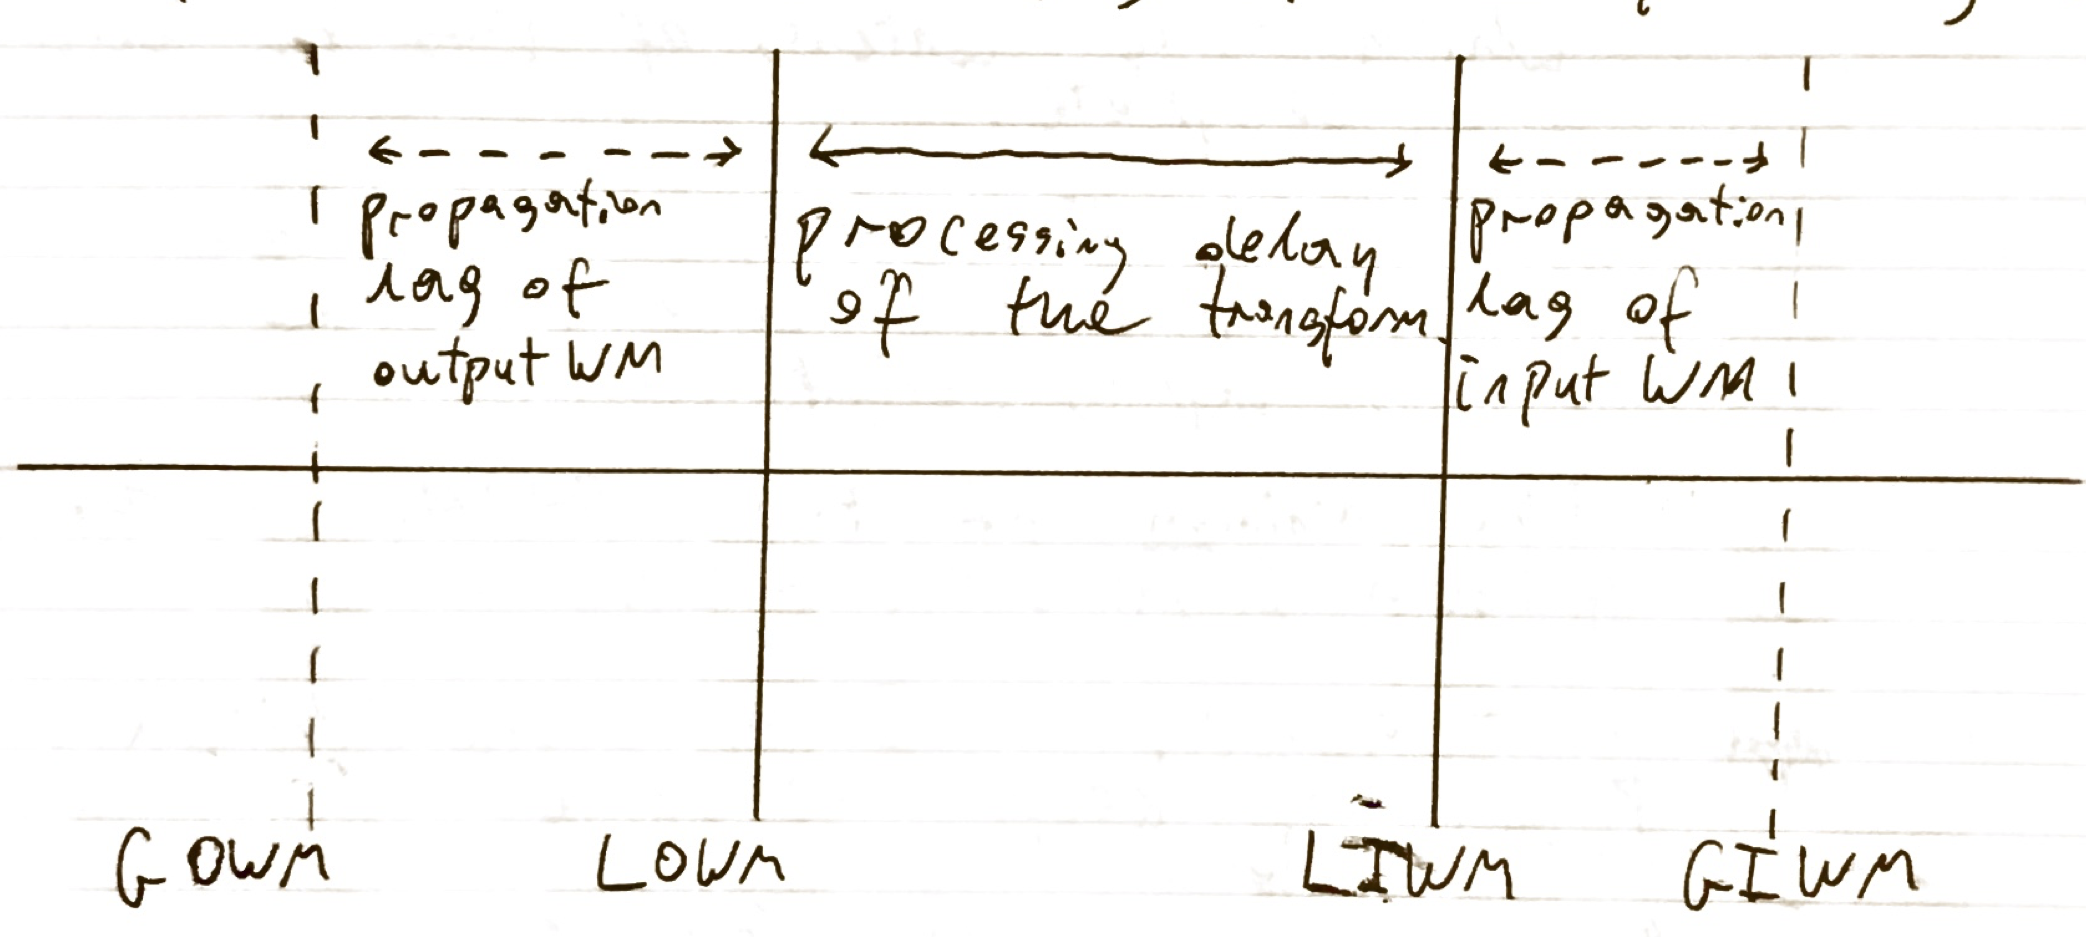
\includegraphics[width=\textwidth]{images/temp/lwm-transform-instantaneous}
	\caption{An instantaneous view of the watermarks of a particular Transform at a single point in processing time.}
	\label{fig:impl:lwm-instantaneous}
\end{figure}

We see that \[ \mathit{GOWM} \leq \mathit{LOWM} \leq \mathit{LIWM} \leq \mathit{GIWM} \] always holds for a particular Transform. \Cref{fig:impl:lwm-instantaneous} illustrates this.

There is also a notion of a \emph{garbage collection watermark}, which is a point in time beyond which it is safe to delete all state we hold about data.
It is usually a constant offset from the local input watermark.
It is not a true component of the Model, but rather an implementation detail necessary to avoid infinitely growing memory consumption.
This concept also limits the amount of lateness we can actually deal with in the system---elements before the GC watermark are silently dropped.
However this is tuneable, so that the user can choose between memory conservation and preservation of late data.

Watermarks provide us with a useful definition of ``doneness''.
In a system where unbounded data may or may not be present, it can be hard to determine when a particular section of the Pipeline is finished and will not receive or output any more data.
We therefore use the watermark to determine this---a watermark of maximal time (infinity) means that we will never receive / output data before that timestamp; since all time is before that timestamp, this implies that we will not receive or output any data at all, and hence we are done.
This is why bounded sources indicate they are done by simply advancing their watermark to the maximal timestamp.

\subsection{``Lateness'' and its semantics}\label{sec:impl:dataflow:lateness}

We have thrown around the term ``lateness'', but so far have failed to define it precisely.
Let us rectify this now.

\todo{evaluate whether using textbf for emphasis is ok or if it's too much}

\textbf{An element added to a Collection is \emph{late} if its timestamp is less than the global watermark of the Collection at the time of the addition, and \emph{non-late}\footnotemark\ otherwise.}

\footnotetext
{
We use \emph{non-late} because \emph{early} and \emph{on-time} have different, discrete, meanings.
}

We say an element is \emph{droppable} when the the garbage collection watermark is after the end of the window to which it belongs; that is, the data is expired and may be dropped at any further point in the Pipeline.

A key invariant in the Dataflow Model which allows us to easily reason about the behaviour of our system is the following:

\textbf{Only late input can result in lateness anywhere in the system.}

This requirement ensures that we always err on the side of marking data as non-late, and only marking it as late if we are certain that it is.
This is because the goal of the system is to avoid lateness where possible, without holding back the progression of the pipeline.
If we have an opportunity to integrate data which is technically late at one stage of the pipeline into output which is non-late at the next, that is a good thing---it essentially takes advantage of the fact that the later part of a pipeline may be progressing more slowly to allow data to ``catch up'' where possible, while also not holding the progress back to wait for potential late elements.

We can define a set of rules that Transforms in the Model must follow which ensure that the above invariant holds.

A complication arises because we only have access to local watermarks, which are mere approximations of the global watermark, in order to do this.
\Cref{fig:impl:lateness-knowability} illustrates the knowability of whether input or output data is late or not, from the perspective of an individual Transform.

\begin{figure}[t]
	\subfloat[][The knowability of the lateness of $t_{\mathit{in}}$ with respect to the $\mathit{LIWM}$.]{
		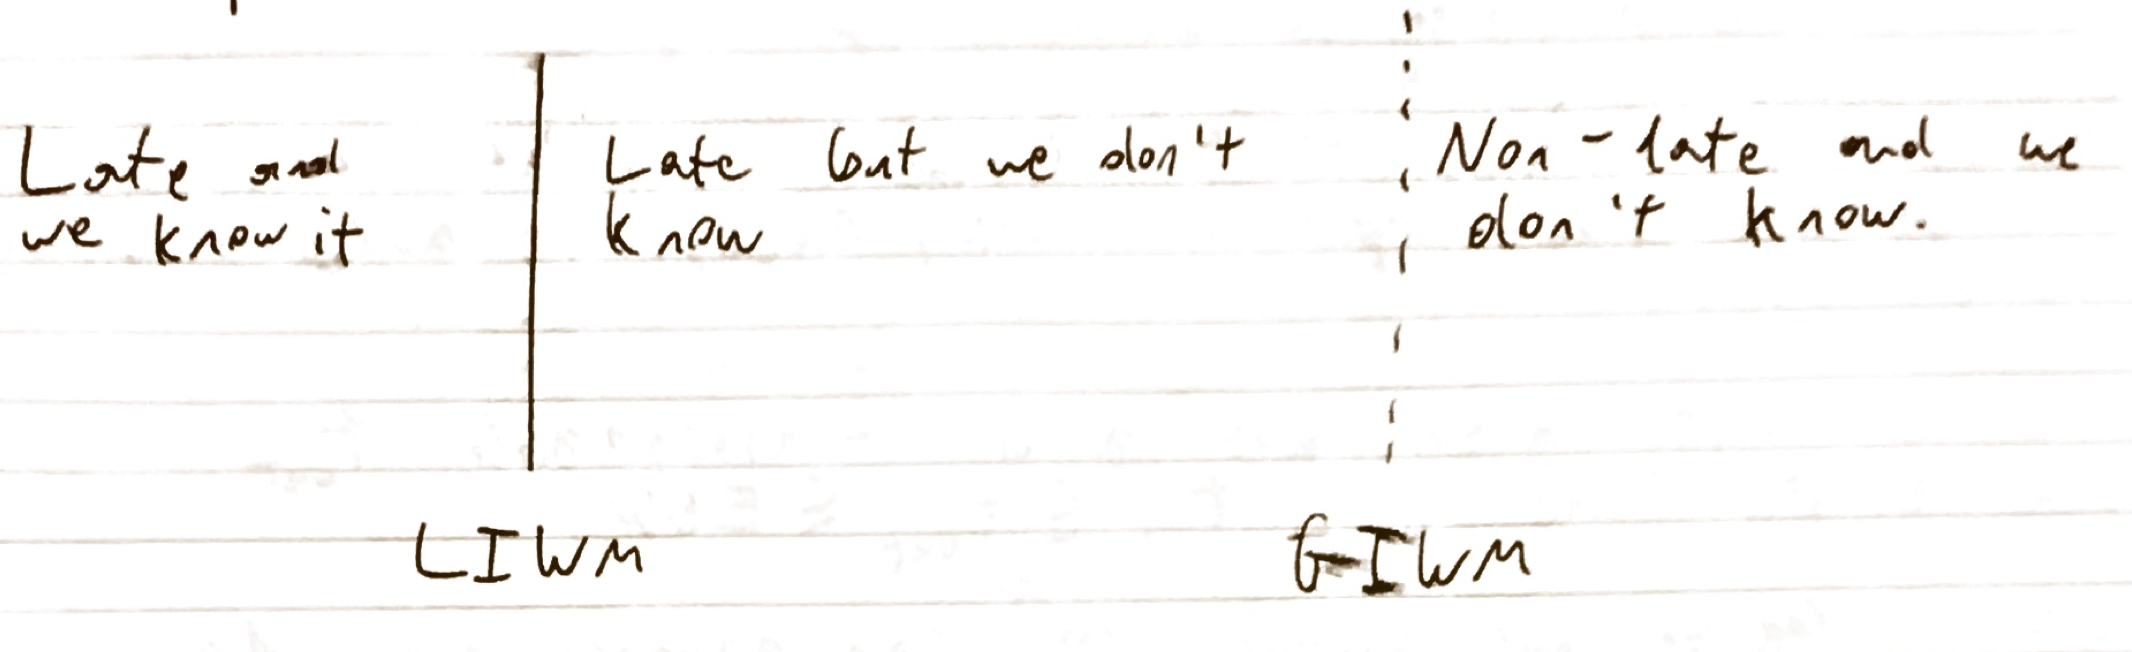
\includegraphics[width=\textwidth]{images/temp/lateness-knowability-input}
	}\\
	\subfloat[][The knowability of the lateness of $t_{\mathit{out}}$ with respect to the $\mathit{LOWM}$.]{
		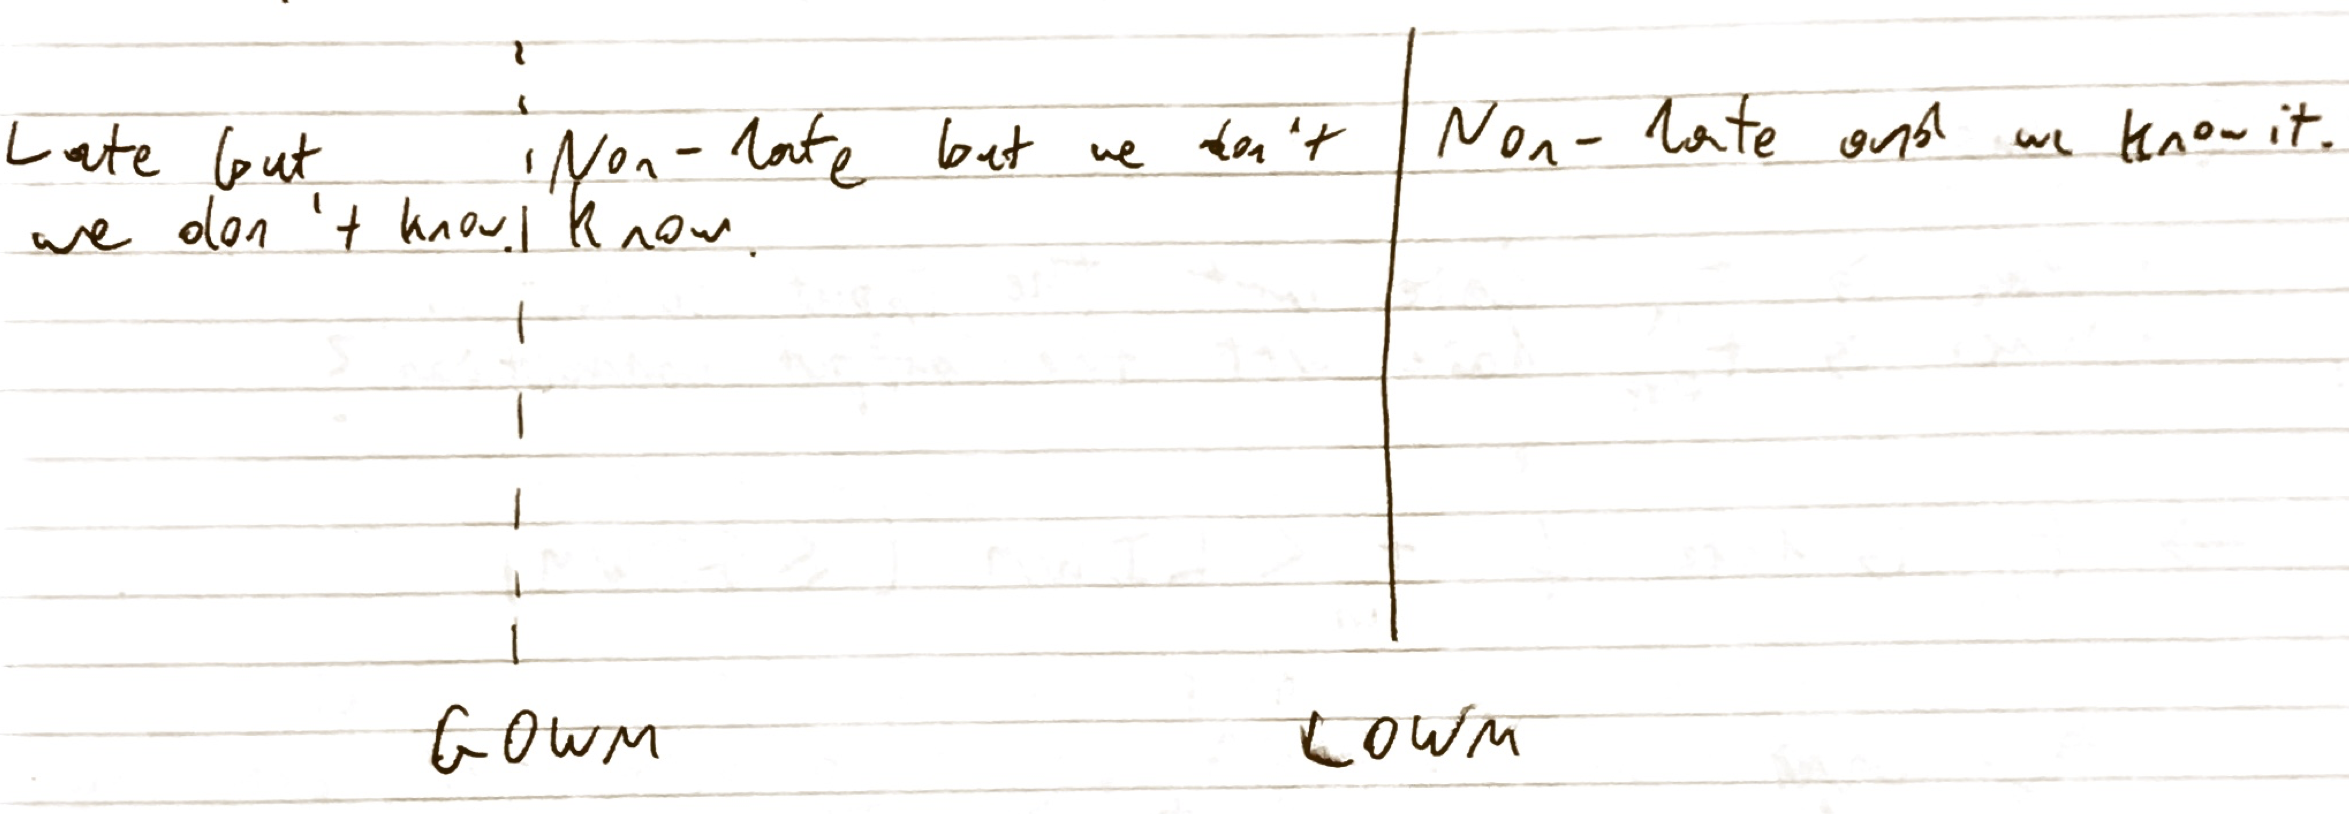
\includegraphics[width=\textwidth]{images/temp/lateness-knowability-output}
	}
	\caption{Diagram illustrating the knowability of the lateness of elements with respect to their position relative to local watermarks.}
	\label{fig:impl:lateness-knowability}
\end{figure}


We therefore expand the original invariants to the following, which ensure the original invariant it is maintained in the situation of imprecise knowledge of the true watermark.

\todo{do we need some sort of informal proof that these actually ensure the original one?}

We then impose the following invariants / requirements on Transforms:
\begin{itemize}
	\item If an element is added to an input Collection non-late, output derived from that element must be added to its respective Collection non-late.
	\item If an element is added to an input Collection non-droppable, then output derived from that element must be added to its Collection non-droppable.
	\item If a pane is emitted, it should not be droppable.
	\item The panes of a window must follow the sequence \verb|EARLY* ON_TIME? LATE*| (zero or more early panes, then zero or one on-time panes, then zero or more late panes).
	\item If a pane is marked early or on-time, it must be non-late in actuality.
	\item If a pane is marked late, it must have been derived \textbf{exclusively} from late input elements.
\end{itemize}

\subsection{Elementwise Transforms}\label{sec:impl:dataflow:elementwise}

\todo{describe ParDo and DoFns}

\subsection{Grouping Transform semantics}\label{sec:impl:dataflow:grouping}

\todo{if short on space, move the details of this section to an appendix, but keep only overall decisions/priorities, and the motivations. This is probably a prime candidate for shortening anyway.}

Keeping in mind that the overall goal is to allow the output watermark to progress as fast as possible without introducing any lateness which was not introduced at the source, an overview of the algorithm every grouping Transform must follow can be defined.

Suppose that we have received an element with timestamp $t_{\mathit{in}}$ which belongs to a particular window $w$ with inclusive upper bound $t_{\mathit{EOW}}$, and it is abut to be buffered for output at a later stage.
The element also has a time $t_{\mathit{out}}$, from which the timestamp of the pane this element will be part of is derived.\footnotemark\ 
This time is such that \[t_{\mathit{in}} \leq t_{\mathit{out}} \leq t_{\mathit{EOW}}\] and is included to allow the advancement of the output watermark even if the current window is not yet ready for output.

\footnotetext
{
Both $t_{\mathit{out}}$ and the derived pane timestamp are controlled by a user-specifiable OutputTimeFn, though in most cases the default of ``use the end-of-window time for both'' is used.
}

For example, with sliding windows, once we are in the context of one particular window (elements can have multiple windows) it is safe to treat the timestamp of an element as the end of the window, because all elements in the window are processed the same and the difference is not observable in the output.
Doing this, however, will allow us to advance the watermark to just before the end of the current window (and new elements in this window will not be late, since we perform the lateness checks on $t_{\mathit{out}}$), allowing earlier sliding windows to close and output their panes with less delay.



We don't want elements that will be output late anyway to hold up the output watermark, except to avoid becoming droppable.

\todo{number the invariants and reference throughout?}

\subsubsection{Lateness}

\begin{figure}
	\centering
	\subfloat[][If $t_{\mathit{in}}$ could be non-late, then $t_{\mathit{out}}$ must be non-late. Similarly, if $t_{\mathit{out}}$ could be late, then $t_{\mathit{in}}$ must be late. If $t_{\mathit{out}}$ is non-late and the $\mathit{LIWM}$ has not reached the end-of-window, $t_{\mathit{out}}$ is on-time.]{
		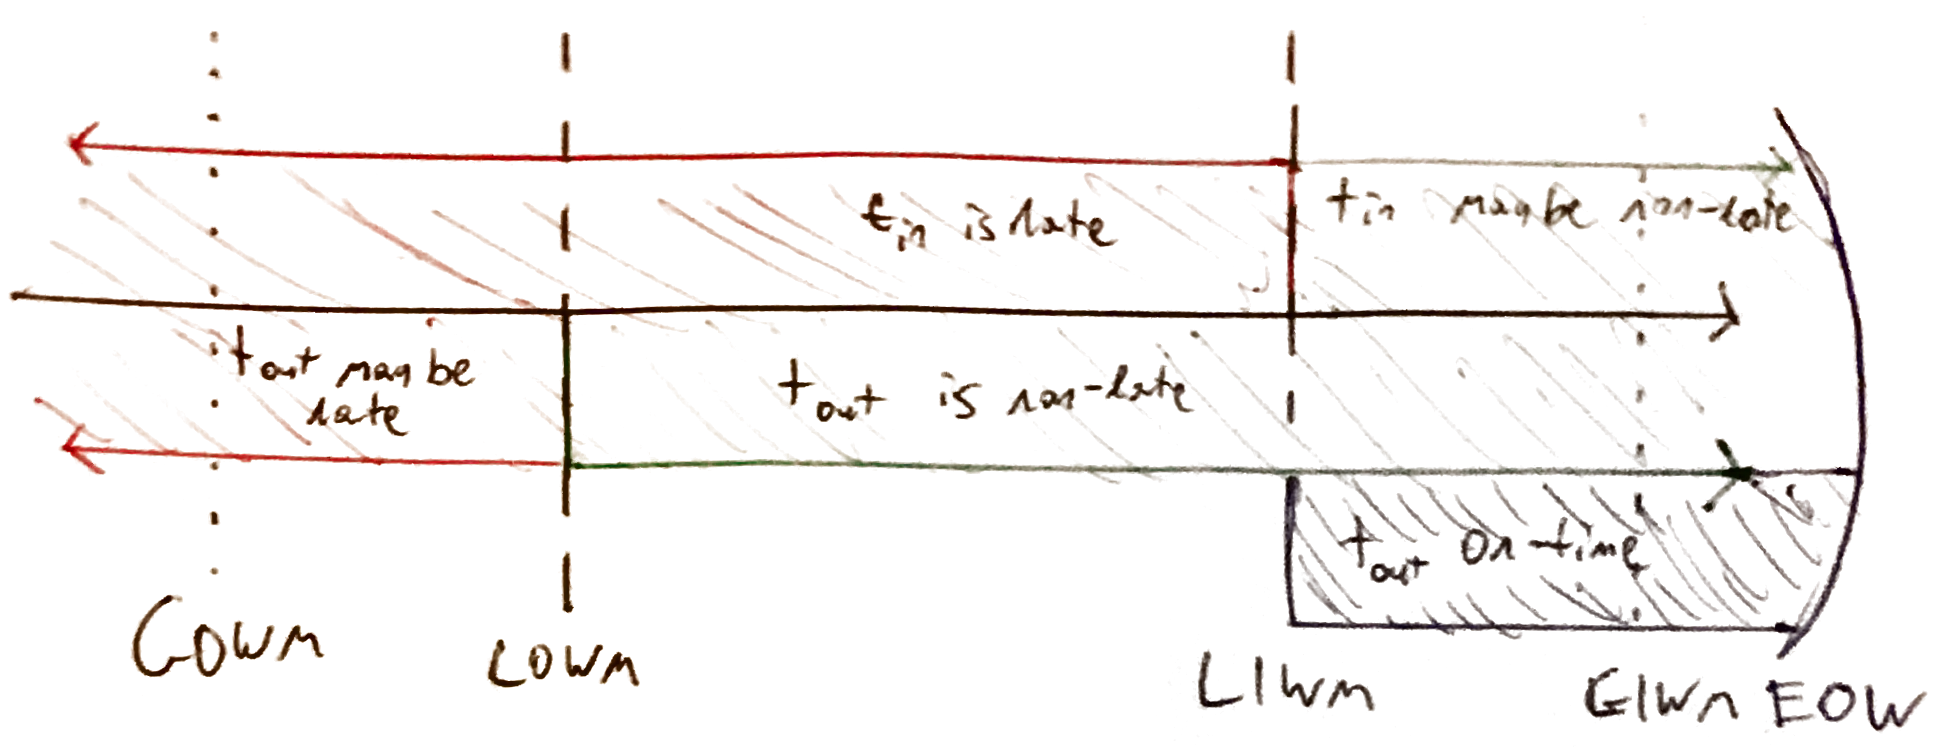
\includegraphics[width=\textwidth]{images/temp/lateness-semantics-1}
		\label{fig:impl:lateness-semantics:a}
	}\\
	\subfloat[][If the $\mathit{LIWM}$ has passed the end-of-window, then $t_{\mathit{in}}$ is definitely late. $t_{\mathit{out}}$ may technically be non-late, but it is not on-time.]{
		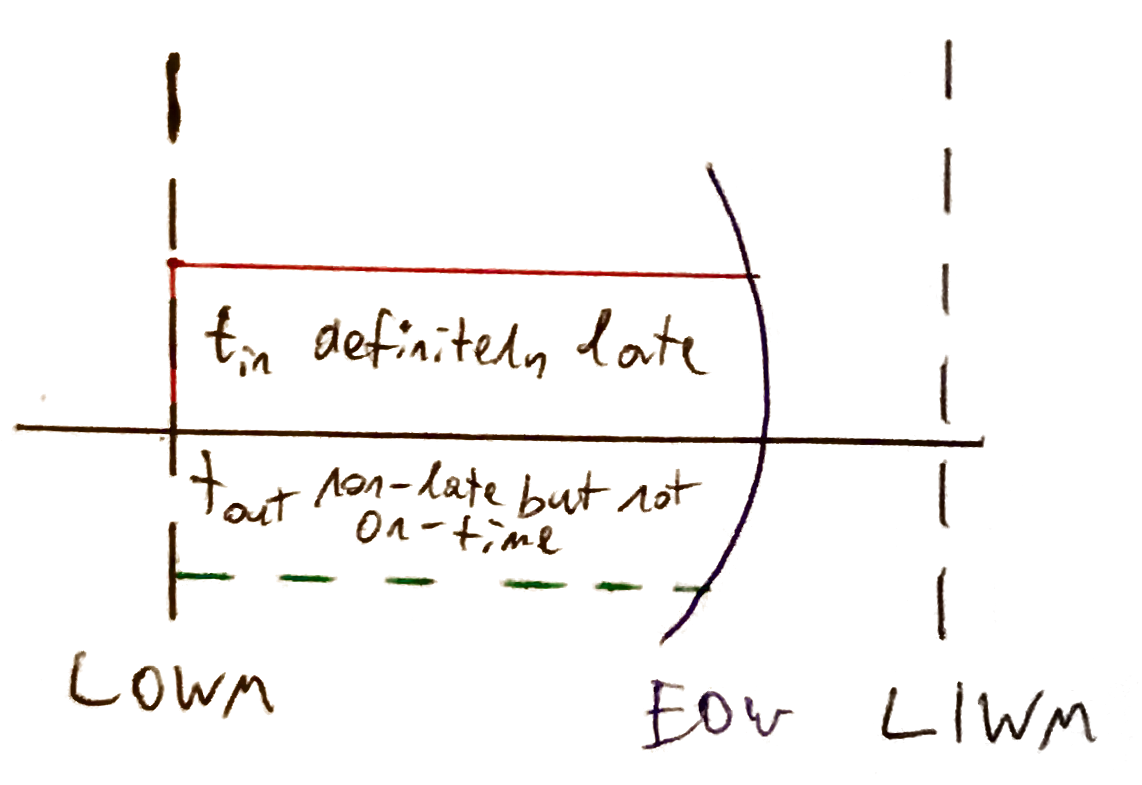
\includegraphics[width=0.5\textwidth]{images/temp/lateness-semantics-2}
	}
	\caption{Diagrams showing regions in event time associated with particular late/non-late or on-time knowledge of $t_{\mathit{in}}$ and $t_{\mathit{out}}$.}
	\label{fig:impl:lateness-semantics}
\end{figure}

There are two questions to answer in order to proceed:
\begin{enumerate}
	\item When is $t_{\mathit{in}}$ late with regards to the input Collection?
	\item When is $t_{\mathit{out}}$ late with regards to the output Collection?
\end{enumerate}

Referring to \cref{fig:impl:lateness-semantics}\subref{fig:impl:lateness-semantics:a} we see that
\begin{enumerate}
	\item \begin{itemize}
	\item $t_{\mathit{in}}$ \textbf{is late} if $t_{\mathit{in}} < \mathit{LIWM}$.
	\item Otherwise, if $t_{\mathit{in}} \geq \mathit{LOWM}$, $t_{\mathit{in}}$ \textbf{could be late} (but we don't know).
	\end{itemize}
	\item \begin{itemize}
	\item $t_{\mathit{out}}$ \textbf{is non-late} if $t_{\mathit{out}} \geq \mathit{LOWM}$.
	\item Otherwise, if $t_{\mathit{out}} < \mathit{LOWM}$, $t_{\mathit{out}}$ \textbf{could be late}. However, in this case, $t_{\mathit{in}}$ \textbf{is definitely late} since $t_{\mathit{in}} \leq t_{\mathit{out}} < \mathit{LOWM} \leq \mathit{LIWM}$.
	\end{itemize}
\end{enumerate}

Note that when $t_{\mathit{in}}$ is late, but $t_{\mathit{out}}$ is non-late, and also $\mathit{LIWM} \leq t_{\mathit{EOW}}$, it is valid with respect to our invariants to treat $t_{\mathit{out}}$ as either late or non-late.
We revisit this choice later.

We have a further requirement for the behaviour of our grouping Transform.
We want to be sure to fire at most one on-time pane.
It \textbf{must} contain all non-late input data up to the end of the window.
It could also contain some late input data which luckily arrived before we emitted the pane (but we do not wait for such data).

To allow us to reason about this, we say that $t_{\mathit{out}}$ is \emph{on-time} if it is non-late, and the input watermark has not yet advanced past its $t_{\mathit{EOW}}$, that is the element arrived early enough to be included in the on-time pane.

\subsubsection{Droppability}

We need to determine two further pieces of information:
\begin{enumerate}
	\item When is the input element droppable?
	\item When is the resulting output going to be droppable?
\end{enumerate}

Denote the allowed lateness used to determine the garbage collection watermark as $\delta$.

$t_{\mathit{in}}$ \textbf{is droppable} if $t_{\mathit{EOW}} < (\mathit{LIWM} - \delta)$.\\
$t_{\mathit{in}}$ \textbf{could be non-droppable} if $t_{\mathit{EOW}} \geq (\mathit{LIWM} - \delta)$.\\
$t_{\mathit{out}}$ \textbf{is non-droppable} if $t_{\mathit{EOW}} \geq (\mathit{LOWM} - \delta)$.\\
$t_{\mathit{out}}$ \textbf{could be droppable} if $t_{\mathit{EOW}} < (\mathit{LOWM} - \delta)$.

Now, if $t_{\mathit{in}}$ \textbf{could be non-droppable} then $t_{\mathit{out}}$ \textbf{is} non-droppable, since \[(\mathit{LOWM} - \delta) \leq (\mathit{LIWM} - \delta) \leq t_{\mathit{in}} \leq t_{\mathit{out}}\;\text{.}\]
Also, if $t_{\mathit{out}}$ \textbf{could be droppable} then $t_{\mathit{in}}$ \textbf{is} droppable, since \[t_{\mathit{in}} \leq t_{\mathit{out}} \leq (\mathit{LOWM} - \delta) \leq (\mathit{LIWM} - \delta)\;\text{.}\]

\subsubsection{Watermark holds}

By default, each Transform Executor outputs a watermark which is equivalent to its input watermark, unless the output watermark is held back by a \emph{watermark hold}.
In that case, the output watermark is the earlier of the two.
Watermark holds provide a mechanism by which the grouping Transform logic can hold back the output watermark until it is sure that it can satisfy the invariants described above.

Each Transform Executor has a watermark manager which maintains a pair of two holds (the data hold and end-of-window/garbage-collection hold) per window\footnotemark.
These are maintained separately so that they can be cleared and manipulated individually, but the overall watermark hold is simply their overall minimum.
Two holds are maintained for each window because some of the logic below requires us to know the data-derived hold even if the hold in effect is derived from the window only.

\footnotetext
{
In the Beam implementation, holds (and other per-window concepts) are per-window-per-key for distribution reasons.
}

The data hold is, in effect, a reduction over all the element timestamps seen so far.
The exact reducing function is determined by the OutputTimeFn in use.
While the default one simply sets all element timestamps to the end of their window---therefore making a reduction redundant as all inputs are always the same---other strategies are available such as ``use the latest timestamp seen so far''.

\todo{diagrams diagrams diagrams}

The EOW/GC hold is a ``fallback'', used when we try to set a hold which cannot be honoured because either the output watermark has already progressed past it, or the input watermark has progressed beyond the EOW and therefore a timer to clear this hold won't be fired.
If we try to set an element hold in either of those situations, we automatically instead try to set the EOW/GC hold instead.

An end-of-window hold is set in two situations:
\begin{itemize}
	\item The element is too late with respect to the output watermark to hold it back, but it may still be possible to include the element in an on-time pane.
	The EOW hold is placed to ensure that pane will not be considered late downstream.
	\item We must ensure that an on-time pane will be emitted for all windows which saw at least one element, even if that on-time pane is empty.
	Therefore, we place the EOW hold to ensure that this (possibly empty) pane will not be considered late downstream.
\end{itemize}

If the input watermark has progressed beyond the end-of-window, we can no longer place the EOW hold since a timer will not fire to clear it.
Instead, if the allowed lateness is non-zero, we try to set an additional garbage collection hold, which is analogous to the end-of-window hold but ensures that the panes we emit are at least non-droppable in the case they must be late.

When the trigger for a window fires, the hold for that window is cleared.
However, a garbage-collection hold may still remain for reasons described above.

It is important to keep in mind that when we talk about ``placing a hold'' below, we actually \emph{attempt} to place an element hold with a particular timestamp, at which point the above checks are performed and the appropriate hold set (or, possibly, no hold is set).
This allows for a decoupling of concerns in the two pieces of logic.

\todo{I do actually think I should reference back to the invariants at each step, saying why it is necessary to maintain them.}

\subsubsection{Transform behaviour}

A grouping Transform does not output panes on receiving input elements, but only when it is triggered.
It can, however, modify its output watermark on receiving elements, and managing this well is crucial to achieve good progress in the Pipeline.

The priorities it adopts, therefore, are:
\begin{itemize}
	\item if it is possible to output data non-late, do that as much as we can;
	\item if process late data and may output late, hold the local output watermark as little as possible (allow it to progress as far as possible);
	\item ensure that the invariants hold and that only a single on-time pane is output.
\end{itemize}

We introduce yet another timestamp for each element, the emission timestamp $t_{\mathit{emit}}$.
It is the timestamp that we actually input into the combination function of the OutputTimeFn to obtain the final timestamp of the resultant pane $T_{\mathit{emit}}$.
This additional transformation affords us the flexibility to combine late data with non-late data to obtain a non-late result.
We require that $t_{\mathit{out}} \leq t_{\mathit{emit}} \leq t_{\mathit{EOW}} + \delta$ where $\delta$ is the allowed lateness.

On receiving each element, then, the Transform Executor must decide:
\begin{itemize}
	\item should the element be dropped?
	\item what hold should be placed on the local output watermark? (see remark above)
	\item what value will be used for $t_{\mathit{emit}}$?
\end{itemize}

\textbf{Case 0: $t_{\mathit{EOW}} < (\mathit{LIWM} - \delta)$}\\
Drop the element.
Since $t_{\mathit{in}}$ and $t_{\mathit{out}}$ are both within the window, they are both certainly droppable and therefore so is the element.

\textbf{Case 1: $t_{\mathit{out}}$ is on-time}\\
We treat the element as non-late.
We set $t_{\mathit{emit}} \coloneq t_{\mathit{out}}$ and place a hold at $t_{\mathit{out}}$.

\textbf{Case 2: $t_{\mathit{out}}$ is not on-time}\\
This is either because $t_{\mathit{out}}$ is possibly late, or because the on-time pane may have already fired.
In either case, $t_{\mathit{in}}$ is definitely late.

We set $t_{\mathit{emit}} \coloneq t_{\mathit{EOW}}$, attempting to shift the element forward in order to possibly include it in an on-time pane.
We could also use the current output watermark for $t_{\mathit{emit}}$, but this would have the effect of significantly holding back watermark progress.
The watermark hold logic described above ensures that the hold is set at $t_{\mathit{EOW}} + \delta$, ensuring we won't produce a droppable pane.

\Cref{fig:todo} illustrates the two situations that are possible in this case. It can be seen that $t_{\mathit{emit}}$ will, in general, be late once emitted, but never be droppable. 
The timestamp used is the latest for the correct window, and the hold used is the latest that prevents dropping.
In this way we allow the watermark to progress in the presence of late data, while ensuring it doesn't become droppable in the process.

\subsubsection{Labelling panes}

\todo{make a typographical distinction between the labels EARLY, ON\_TIME, LATE and the late / non-late state of the elements themselves.}

\todo{explain why the labels are needed and how they're used.}

When a grouping Transform Executor is triggered and outputs a pane (again, simply an element of the output Collection), it must label it as either early, on-time or late.
It does this based on the state of the watermarks and $T_{\mathit{emit}}$, the combined output timestamp determined by the OutputTimeFn from all individual $t_{\mathit{emit}}$ values.
It also determines whether a pane is \emph{final}, which lets the downstream know that no more panes for this window will be emitted (as they would have been emitted droppable).

Since a pane is simply another element, the standard definition of lateness applies.

Therefore if $T_{\mathit{emit}} \geq \mathit{LOWM}$, it is non-late.
By design, every $t_{\mathit{out}}$ that went into the pane was non-late as well.

If $T_{\mathit{emit}} < \mathit{LOWM}$, it is possibly late (it could be on either side of the $\mathit{GOWM}$).
By design, this means that at least some of the $t_{\mathit{out}}$ were treated as late, meaning the corresponding $t_{\mathit{in}}$ were certainly late.
In this case, it is appropriate to output this pane element late and label it late if we need to.

The pane can be marked on-time if $T_{\mathit{emit}}$ is non-late, and if $\mathit{LIWM} > EOW$.
This is because any elements which come in after this condition holds will be treated as late, meaning that they do not need to be included in the on-time pane.
They may still be included in this pane if they arrive before we output it, but we do not have to wait for them, since they were produced late to begin with.

The pane is marked final if $\mathit{LIWM} - \delta > t_{\mathit{EOW}}$, since any incoming elements after this condition starts to hold will just be dropped.

Therefore the pane is labelled as follows:
\begin{itemize}
	\item If $T_{\mathit{emit}}$ is possibly late, label it late.
	\item If $T_{\mathit{emit}}$ is non-late, label it on-time is possible, and early otherwise.\footnotemark
	\item Additionally, label the pane as final if appropriate.
\end{itemize}

\footnotetext
{
Note that in the presence of window merging, two or more on-time panes may end up being emitted for the same data.
The ``one on-time pane'' condition holds only per unique window, and so once the window is merged to become another window, the condition holds separately for this new window.
}

\subsubsection{OutputTimeFn}
Grouping Transforms aggregate element data into an output value.
They must also aggregate the elements' timestamps into a single timestamp used for the output pane.
This concern is often orthogonal to the type of data transformation being performed, and so the Model allows its specification orthogonally, through the use of OutputTimeFns.

An OutputTimeFn specifies three aspects of the aggregation:
\begin{enumerate}
	\item how $t_{\mathit{in}}$ maps to $t_{\mathit{out}}$;
	\item how multiple $t_{\mathit{emit}}$ timestamps combine to give the pane timestamp $T_{\mathit{emit}}$;
	\item how multiple tentative $T_{\mathit{emit}}$ values are combined when two windows merge.
\end{enumerate}

There are two obvious approaches for the first aspect---the identity mapping and simply shifting element timestamps to the end of their window.
Other mappings may also be useful.
For example, when using sliding windows we could shift timestamps just past the end of the previous sliding window, allowing it to close.
The default behaviour in general is to output at the end of the window.

Within a single window, we combine the $t_{\mathit{emit}}$ values generated for each element to obtain the final $T_{\mathit{emit}}$ value for the pane.
An OutputTimeFn specifies an associative, commutative function which can reduce the former to the latter.
It must also ensure that $T_{\mathit{emit}} \geq \max(t_{\mathit{emit}})$ so that non-late inputs are not made late by shifting their timestamps backwards.

The default choice is to, again, use the end-of-window time.
It is simple, efficient and easy to reason about.
However, if the input timestamps are to be stored within the pane and then re-used later by generating new elements with those timestamps, we may use the minimum timestamp of all non-late elements seen so far.
This will hold back the output watermark so that we can once again re-use the input timestamps without them becoming late.

When windows merge, the aggregated pane timestamps must be combined too.
The result of accepting elements into two windows and then merging them should be the same as merging first and then combining new elements into the resultant window.
In general, the merge function either behaves the same as the combination function, or does not use its input at all, again using the end-of-window time (the default).

\subsection{Triggers and timers}\label{sec:impl:dataflow:triggers-timers}

In the previous section, we explored how grouping Transforms accumulate data, ensure that their output watermark is held back until the aggregate is output, and mark their output appropriately to let the downstream know of the type of pane emitted.
However, it is still not clear how exactly they know when they should produce some output at all.

The Model's answer to this is the trigger system.
Triggers were introduced in \cref{sec:prep:dataflow:when}, but this section aims to expand on their semantics and how they function to produce the desired behaviour.

\subsubsection{Triggers as state machines}
Once again, we draw the distinction between triggers at Pipeline-construction time, where they are simply bundles of configuration, and triggers (trigger drivers) at execution-time, where they do real work.
In this second case we can think of triggers as finite state machines; indeed, the Beam implementation places its trigger logic in classes extending \verb|TriggerStateMachine|.

A trigger state machine is instantiated per-window (per-window-per-key in Beam) and is used by the main Transform Executor to make decisions on when to output.
We say that a trigger \emph{fires} when it instructs the Transform Executor to output a pane.
Note that a trigger firing is binary---if it fires, all the currently accumulated data is output into a pane, which is timestamped and marked appropriately as detailed below.

We can easily see the overall behaviour of the FSM by looking at the \exs{TriggerDriver} behaviour from the Elixir implementation in \cref{lst:impl:trigger_driver}.\footnotemark

\footnotetext
{
This listing uses the Elixir behaviour/type syntax. A brief overview is available in \cref{todo}<appendix B>.
}

\begin{listing}[h]
	\begin{minted}{elixir}
defmodule Dataflow.DirectRunner.ReducingEvaluator.TriggerDriver do
  alias Dataflow.Utils.Time
  alias Dataflow.{Trigger, Window}
  
  @opaque state :: any
  @callback init(Trigger.t, Window.t, timing_manager :: pid) :: state
  @callback process_element(state, Time.timestamp) :: state
  @callback merge([state], state) :: state
  @callback should_fire?(state) :: boolean
  @callback fired(state) :: state
  @callback finished?(state) :: boolean
end
	\end{minted}
\caption[The \exs{TriggerDriver} behaviour showing the FSM design of an execution-time trigger.]{The \exs{TriggerDriver} behaviour showing the FSM design of an execution-time trigger. The \exs{timing_manager} passed to the \exs{init} function is the \exs{pid} of the current Transform's timing manager, allowing the trigger driver to set and clear timers and access current watermark state.}
\label{lst:impl:trigger_driver}
\end{listing}

\todo{Consider using the Elixir type syntax everywhere in this chapter to specify the different structures being talked about (instead of prose)}

There we see that the FSM is first initialised (\exs{init/3}) with trigger and window data (along with a handle to a process which allows it to set and clear timers asynchronously, as well as read the watermarks and processing time).
It then receives a series of \exs{process_element/2} calls, receiving the timestamps of elements being processed and being allowed to update its state.
It will optionally be asked to \exs{merge/2} its state with that of other windows---typically we require that the actual trigger being used is the same in all cases.

Note that the trigger driver itself does not asynchronously notify the transform executor of its firing.
Instead, the transform executor will ask the trigger driver if it is ready to fire using \exs{should_fire?/1}.
If so, a pane of output is produced and the trigger driver is notified via the \exs{fired/1} callback.

A trigger is \emph{closed} or \emph{finished} if it will never fire again.
The trigger driver can be asked if it is finished using the \exs{finished?/1} callback.
At that point it is safe to garbage collect the associated window state (including the trigger state itself), leaving only a tombstone indicating that new elements placed in this window should be ignored (since they would never have led to output anyway).

It is clear that this model allows great flexibility in specifying exactly when output should occur.
The FSM can count elements, set timers for particular event or processing times, and flexibly decide if it will fire multiple times.
The model could also quite easily be extended to support punctuations (data-driven triggers) by allowing \exs{process_element/2} to inspect the element value itself.
This is not implemented, but being worked on, in Beam (as certain implementation difficulties arise there) and was considered out-of-scope for the Elixir implementation.

It should be noted that a standard pattern in the Model is to use composite triggers---for example, a trigger which fires when trigger A \emph{or} trigger B fire, or one which takes a one-time firing trigger A (one which becomes finished after firing once) and instead resets it after each firing, making it able to fire indefinitely.
This is enabled by the decouple design of the trigger drivers, allowing them to be queried by a ``parent'' trigger just as easily as they could be queried by the transform executor itself.

\subsubsection{Example: The default trigger}

The \emph{default trigger} used when no other trigger is explicitly specified fires once when the event watermark passes the end-of-window, and fires again every single time a late element is seen (producing a one-element late pane with that element).

\Cref{lst:impl:default_trigger} illustrates the simple logic needed to accomplish this behaviour.

\todo{the listing is about 60 lines of code total including liberal line breaks for readability and comments. possibly skip it here though, maybe just include the pseudocode of the logic?}

\subsubsection{Timers}

Timers are a very simple, but yet flexible way to schedule asynchronous action in the future.
A timer is simply a tuple of \exs{{namespace, time, domain}}\footnotemark, with the \exs{domain} being one of \emph{processing time} or \emph{event time}.
A timing manager is instantiated per transform executor, though it operates asynchronously to the transform executor itself.
It handles watermark management and timers.

\footnotetext
{
In Beam, timers also have a unique ID, in order to identify and compare their identity. This is not needed in Elixir, since they can be directly compared value-wise.
}

Once a timer is set, the timing manager will notify the transform executor once it fires.
This will happen when the input watermark (event time) or clock time (processing time) \textbf{passes} the time of the timer; that is, when the appropriate time measure is strictly greater than the time of the timer.
An exception is a timer for the maximal event time, which fires precisely when that time is reached, since it cannot advance past it.
Multiple timers may fire simultaneously, and the transform executor will be notified of all of them.

The \exs{namespace} of a timer is an arbitrary value, but in practice is used to associate timers to the triggers that set them, or to keep track of different timer purposes in more custom implementations.
Often (e.g.\ in the grouping Transform) the namespace is not even read on a timer firing (all timers are treated the same), but rather only employed to clear specific timers before they fire.

It is important to note that no semantics are implied by the timers themselves---they simply provide a mechanism to receive a notification with a particular identifier at a particular time.
It is up to the transform executor to interpret this and act accordingly.

In the case of a grouping Transform, the executor simply asks the trigger driver whether it should fire already.
The trigger has access to the current watermark state, and so can determine whether it is time to fire.
The flexible implementation means that it could just as well set another timer at this point, enabling strategies such as ``output a pane every five seconds until the end of the window, but only if we've seen 10 elements or more''.

\subsection{Watermark generation and processing}\label{sec:impl:dataflow:watermark-generation}

\todo{diagram}

In \cref{sec:impl:dataflow:lateness} it was asserted that only late input can result in late data anywhere in the system.
Late input was also defined as that whose timestamp falls behind the current input watermark.
The previous sections also detail the exact semantics necessary to preserve watermark correctness along with many useful invariants throughout the whole Pipeline.

However, none of the preceding sections address the question of generating some watermark ``from nothing'' in the first place.
This process is crucial---as mentioned above, it is the only part of the system in which lateness can be introduced.

It also very application-specific.
A watermark is an indication of the progress made so far in the event stream.
For some data sources, we can get a guaranteed-correct position in the stream that we have read up until.
For others, the source provides us with only an approximations.
In yet other cases, we must keep statistics about the source to generate a heuristic ourselves.

Clearly there is no standard solution---there must be a mechanism to allow flexibility in watermark generation.
We introduce the standard concept of a \emph{Source}, which can provide a Collection from some external source when coupled with a \verb|Read| Transform.

At execution, the \verb|Read| Transform Executor will use logic found in the Source it is given in order to assign timestamps to elements being read (usually an intrinsic timestamp in the case of e.g.\ Kafka messages) and to publish a watermark using any logic and state it needs to, with the only restriction being that it must be monotonically increasing.
Bounded sources with no intrinsic timestamps will generally output a minimal watermark (and timestamp all output with the minimal timestamp) until it is finished, advancing the watermark to the maximal timestamp to indicate that.

Sources for popular data sources such as the file system, Apache Kafka, Google BigQuery and others are included in the Beam implementation, and an API is provided to add custom ones with arbitrary watermark logic (in fact, this API is utilised for the example used in \cref{sec:eval:todo}).

\subsubsection{Watermark domains}

Forcing the Source to generate the original input watermark works well from a system perspective, providing a single, easily-managed point where lateness can be introduced.
However, it can cause problems from a user perspective and limit the flexibility of the Model.

Suppose a Pipeline is receiving data containing names of log files being saved off to some cloud storage.
These files contain log entries collected during a particular day, which are then dumped to storage during log rotation every 24 hours.
The timestamp of these elements will be the timestamp of the file, which will be \textbf{after} all of the entries in the file.

This means that if we were to process the file contents in a Transform and output all the log entries within as individual elements, all those elements would have to be output late if they kept their real timestamps.
They could avoid being dropped by selecting an appropriate value for the allowed lateness, but that is a misuse of the Model and semantically incorrect.

In fact, these new elements are not late, because they belong in a different \emph{watermark domain} than the files containing them.
Collections can be thought of as being in the same watermark domain when their elements' timestamps directly relate to one another \textbf{independently of the element data}.
For example, when extracting body text from a social post, it makes sense to assign the same timestamp to the text as was assigned to the post itself.
We don't need to actually look at the post to make that decision.
Similarly, a grouping Transform treats data aggregation and timestamp aggregation orthogonally.

\todo{diagram}

However, in the log-file example given, the timestamp of an individual log entry generated from a file will be dependent on the data of the log entry itself---the recorded time of its generation.
We may be able to provide a guarantee such as ``the timestamp of an entry will never be earlier than 24 hours before the timestamp of a file'', but this again is an application-specific decision, unsuitable for inclusion in a generic Model.
Such a guarantee also constitutes precisely what a watermark is.
Alas, in order to have a predictable lateness model, we have constrained the output watermark of a Transform to always be less than or equal to its input watermark.
Shifting our watermark to 24 hours before the input watermark would violate this invariant.

The solution is to break our Pipeline apart into watermark domains.
The invariants and relationships described in this chapter hold only within one watermark domain---we are essentially treating each one of these as a mini-Pipeline of its own.

Just how event time and processing time are distinguished, we now treat event time as a \emph{class} of domains rather than a single domain of its own.

The lateness semantics only make sense when applied to data which can all be semantically described with one time domain.
Once we switch semantic time domains, there is no general algorithmic solution to obtaining the correct watermark---the problem becomes once-again application-specific.
This is the same problem faced when considering the initial input data into the Pipeline, and so it makes sense that it be solved similarly.

It is to introduce the concept of a Transform which initiates a new watermark domain.
These transforms may directly manage their own input watermark, which does not need to (but can) have a direct relation to their input watermark.

This, of course, introduces a potential source of lateness at every point such a Transform is placed in the Pipeline.
However this also semantically makes sense.
At these points, we are essentially reading a conceptually new, external Collection of elements, with timing information which did not ``exist'' in the Pipeline until this point.
Since this information is unavailable before this point, it is impossible for the previous transformations to have taken account of it in determining whether input to the system was late.

The watermark domain solution is the proposal of the author and is not in place in the Beam Model.
It is included in the Elixir implementation of the Model.
There is no accepted general solution to this problem in the Beam community.

The proposed solution also potentially simplifies the original approach to Sources.
An example of this can be seen in one of the Evaluation examples (\cref{sec:todo}).


\section{The Dataflow Model implemented}\label{sec:impl:approach}

\subsection{The Dataflow DSL}\label{sec:impl:approach:dsl}

An important component of this project, and one of its original goals, was the design of a readable, approachable DSL for constructing pipelines.

As described in \cref{todo}, Elixir has a widely-used pipeline operator \exs{|>}, and programmers are encouraged to express their programs using series of data transformations.
Thus, the Dataflow way of expressing computation translates quite naturally into Elixir, and only a minimal amount of additional syntax is necessary.

\begin{listing}[h]
	\caption{An example of Pipeline construction in Elixir. A Pipeline is created, and to it are applied Transforms which count the words in a file and output these counts to a new file. The Pipeline is then executed.}
	\label{lst:impl:elixir-construct-pipeline}
	\begin{minted}{elixir}
use Dataflow
alias Dataflow.Transforms.{Core, IO, Aggregation}
alias Dataflow.DirectRunner

pipeline = Pipeline.new

pipeline
~> IO.read_file("data/data1.txt")
~> Aggregation.count_elements()
~> "Format Counts" -- Core.map(fn {word, count} -> "#{word}: #{count}" end)
~> IO.write_file("data/output.txt")

DirectRunner.run pipeline, sync: true

	\end{minted}
\end{listing}

\Cref{lst:impl:elixir-construct-pipeline} illustrates the API with a very simple, but working example.
We read a file which contains a single word on each of its lines.
We count the number of occurrences of each word, format this information and output it to another file.

The code is clear and understandable, and maps very well to the Elixir model of data processing.
\Cref{fig:todo} shows this Pipeline as a DAG.

In line 10, we see the \exs{--} operator being used to assign a label to a particular Transform.
Assigning labels to transforms is an important feature, very useful for managing and visualising Pipelines.
This notation evokes the use of \verb|--| to denote a dash in \LaTeX.

\begin{listing}[h]
	\caption{An implementation of the process in \cref{lst:impl:elixir-construct-pipeline} using regular, sequential functions.}
	\label{lst:impl:elixir-normal-comparison}
	\begin{minted}{elixir}
input = File.stream!("data/data1.txt")
output = File.stream!("data/output.txt", [:write])

input
|> count_elements() # helper function
|> Enum.map(fn {word, count} -> "#{word}: #{count}" end)
|> Enum.into(output)
	\end{minted}
\end{listing}

\Cref{lst:impl:elixir-normal-comparison} shows, for comparison, how this process would usually be implemented using normal, sequential processing in Elixir.
The most obvious difference between this listing and \cref{lst:impl:elixir-normal-comparison} is that in the latter, we include an extra \exs{pipeline} identifier which has to explicitly be \exs{run}.
This makes sense, as the Model requires us to separate the description of the computation in the construction phase from its execution in the subsequent phase.

\subsubsection{Using macros}

Those with a passing familiarity with Elixir will recognise that \exs{--} is actually the list difference operator.
While it would be possible to have the \exs{use Dataflow} statement replace the default \exs{--} with a version used for labelling Transforms, it would likely cause confusion.
How then is this entire syntax implemented?

The answer is that \exs{~>} is in fact a macro.
Elixir macros are powerful tools, allowing arbitrary AST transformation at compile time.
They can also cause unexpected behaviour and confusion, and the convention is to keep their use minimal, relying on functions instead.
This is why the definition of \exs{~>} is only a few lines long, shown in \cref{lst:impl:elixir-dpipe-macro-def}.

\begin{listing}[h]
	\caption{The definition of the \exs{~>} macro, showcasing the usefulness and power of Elixir macros.}
	\label{lst:impl:elixir-dpipe-macro-def}
	\begin{minted}[autogobble]{elixir}
 defmacro pvalue ~> transform_with_label do
    case transform_with_label do
      {:--, _, [label, transform]} ->
        quote bind_quoted: [pvalue: pvalue, transform: transform, label: label] do
          Dataflow.__apply_transform__(pvalue, transform, label)
        end
      transform ->
        quote bind_quoted: [pvalue: pvalue, transform: transform] do
          Dataflow.__apply_transform__(pvalue, transform)
        end
    end
  end
	\end{minted}
\end{listing}

Macros are simply functions which, at compile-time, take the Abstract Syntax Trees (ASTs) of their arguments and output an AST with which they are replaced.

The \exs{~>} macro works by pattern-matching on the structure of the second argument, which will either be an AST node of the form \exs{label -- transform} (line 3) or something else (line 7).
The macro outputs a new AST node which simply calls the \exs{Dataflow.__apply_transform__} function which contains the Transform application logic.
This matching at the AST level means that we are free to assign \exs{--} a new meaning only within this expression, without needing to shadow the original meaning for the entire namespace.

Note that we do not have to manually construct this node---the \exs{quote} macro allows us to create one by simply writing syntax and specifying which variables from the macro's environment we want to bind to the environment of the resultant AST node (the \exs{:bind_quoted} option).

The only other piece of ``magic'' present is that the \exs{use Dataflow} line imports the \exs{~>} macro into the top-level namespace so that it can be used straight away.
In fact, that line of code simply calls the \exs{Dataflow.__using__} macro.
In this way, Elixir allows developers to strike a good balance between friendliness and ease-of-use, and the lack of magic and explicitness which is very desirable when things go wrong.

Intuitively, the result of an application of the \exs{~>} operator is a Value, which is either a Collection or some compound (e.g.\ a tuple) containing Collections.
We can hold on to Collections that are returned in this way and apply Transforms to them several times.
This means that we can create branching Pipelines such as the one in \cref{fig:todo} easily, as shown in \cref{lst:impl:diverging-pipelines}.

Note that in order to instantiate a root Transform (one which produces data obtained outside the system somehow), we apply it to the Pipeline itself.

\begin{listing}[h]
	\caption{An example of the creation of a branching Pipeline.}
	\label{lst:impl:diverging-pipelines}
	\begin{minted}[autogobble]{elixir}
pipeline = Pipeline.new

words =
  pipeline
  ~> IO.read_file("data.txt")
  ~> extract_words()
  
# save words to file
words ~> IO.write_file("words.txt")

# also get the top words and write them to another file
words
~> get_top_words()
~> IO.write_file("top_words.txt")
	\end{minted}
\end{listing}

\subsubsection{Structs and protocols}

Since there is a need to separate the construction and execution phases of the Model, the situation cannot be as simple as in \cref{lst:impl:elixir-normal-comparison}, where on passing a value to a ``transformation'', we simply call the function directly.
Instead, we must store the description of the computation in the Pipeline structure.

In order to facilitate this, we make use of Elixir's protocols and structures.
A structure is simply a map with a special \exs{:__struct__} key, which exhibits some special behaviour at compile-time.
A structure is always associated with a particular module.

A protocol is an interface module consisting of a set of functions.
Implementations of a protocol can then be defined on a per-module basis, as long as that module declares a structure.
When the protocol functions are then called with a structure whose module implements that protocol, the actual function called will be dynamically dispatched to that module.

The functions in the example listings, such as \exs{IO.read_file/1}, don't actually perform any computation themselves---instead, they return a structure which stores the arguments passed in and implements the \exs{PTransform.Callable} protocol.
For examples, the result of calling \exs{IO.read_file("data.txt")} is \mintinline{elixir}{%IO.ReadFile{filename: "data.txt"}}.

We then see from the definition of \exs{~>} in \cref{lst:impl:elixir-dpipe-macro-def} that these structures are incorporated into the Pipeline by calling the appropriate function which internally uses the protocol.

The definition of the protocol is presented in \cref{lst:impl:ptransform-callable}.
We see that the only requirement is for the Transform to be able to expand to more Transforms, following the Composite Transforms concept introduced earlier.
Primitive Transforms are not definable by the user and receive special treatment, but the user is free to define their own Composite Transforms by providing an appropriate structure and module, much like one would define small, composable functions.
It is technically possible to simply use a function which composes Transforms internally, but this means that this new Transform is not recognised as a node, leading to a poorer experience once visualisation and/or reporting is introduced.

\subsubsection{Managing DAGs using asynchronous processes}

\todo{ref to a paper on implementing functional dags in Haskell?}

Constructing and working with DAGs in the absence of mutability, especially when advanced functional features such as those found in e.g.\ Haskell are not available, lies somewhere between impossible and infeasible.
Instead of attempting to do this, we leverage the concurrency model of Elixir to simulate a mutable map of Collections and Applied Transforms inside the Pipeline structure.

\todo{mention that Erlang's :digraph library also uses mutable state but is unsuitable for use here?}

The call to \exs{Pipeline.new} actually starts a new process which contains a map of the Collections (edges) and Applied Transforms (nodes) in the Pipeline graph, indexed by a unique integer ID.
This means that it is possible to easily add new structures to the DAG, even in the face of Composite Transforms or branching Pipelines.

It is clear from \cref{lst:impl:diverging-pipelines} that Pipelines behave like mutable objects---merely using the \exs{~>} operator on a Pipeline modifies it.
Therefore Pipelines in this state are better thought of as processes rather than values.
However, once the construction of the Pipeline is finished, it is possible to ``freeze'' it and turn it into a simple data structure which once again behaves in the expected manner.
Indeed, the \exs{DirectRunner.run} function does this internally before taking this data structure and executing it.

\subsection{Making state explicit}\label{sec:impl:approach:state-explicit}

\todo{discuss moving from a stateful approach where things can just grab state out of thin air and mutate it, into an explicit approach of functions taking state and returning a modified version of the state. Also expand on how this forces greater focus on what a particular function actually does as it needs to explicitly receive things it needs, and explicitly return things it touches/modifies.}

\subsection{Managing concurrency with OTP and GenServers}\label{sec:impl:approach:concurrency}

\todo{Introduce the concept of OTP, GenServers and how they provide robust, serialised concurrency. Make clear how building on top of these core libraries is advantageous and appropriate. Mention how clear semantics enable concurrency design.}

\subsection{The GenStage library}\label{sec:impl:approach:genstage}

\todo{Introduce concept of GenStage and how it builds on GenServer. Mention how its operation is a great fit for the type of computation being done in Dataflow.}

\subsection{Extensibility using behaviours and protocols}\label{sec:impl:approach:extensibility}
